% +------- CÓDIGO FONTE TCC -------+
% 	Autor: Arllem Farias, 2017.
% 	E-mail: arllemfarias@ufam.edu.br
%   Revisor: João Victor Lima Lopes
%   E-mail: jvllopess@gmail.com
% +--------------------------------+

% Ítens como: Ficha Catalográfica, Folha de Aprovação Assinada e Lombada, devem ser adicionadas posteriormente
% e descomentar as linhas que as adicionam (Linhas 132,134 e 135).

% Classe do documento --> \documentclass[OPÇÕES]{CLASSE}
\documentclass[
			   a4paper, % Tipo de papel 
			   oneside, % Impressão em apenas um lado da folha
			   12pt     % Tamanho da fonte
			   ]{book}  % Classe do documento

% Pacotes --> \usepackage[OPÇÕES]{PACOTE}
\usepackage[utf8]{inputenc} % Codificação do documento (conversão automática dos acentos) 
\usepackage[brazil]{babel}  % Traduz palavras chaves para o PT-BR (ex.: abstract->resumo)
\usepackage{indentfirst}    % Indenta o primeiro parágrafo de cada seção
\usepackage{setspace}		% Possibilita a alteração do espaçamento entre linhas
\usepackage{graphicx}       % Possibilita a inserção de figuras
\usepackage{subcaption}     % Possibilita a inserção de subfiguras
\usepackage{pdfpages}       % Possibilita a inserção de páginas em pdf
\usepackage{amsmath}        % Inclui funções adicionais no ambiente matemático \eqref{•} \dfrac{•}{•}
\usepackage{amssymb} 		% Símbolos adicionais no documento \mathbb{R}
\usepackage{amsfonts}
\usepackage{amsthm}
\usepackage{mathrsfs}       % Símbolos da transformadas de Laplace e Fourier \mathscr{•}
\usepackage{float}			% Possibila posicionar tabelas e figuras em uma posição específica [H]
\usepackage[numbers]{natbib}% Inclui mais possibilidades de citações \citep{•}
\usepackage{fancyhdr}       % Possibilita a alteração de cabeçalho e rodapé
\usepackage{longtable}      % Possiblita a quebra de tableas em duas páginas
\usepackage{multirow}		% Possibilita multiplas linhas em tabelas
\usepackage{array}			% Possibilita o uso do comando \newcolumntype{•}[•]
\usepackage{pdflscape}      % Possibilita a inserção de páginas em modo paisagem
\usepackage{listings}		% Possibilita inserir códigos fontes (C++, Java, ...)
\usepackage{slashbox}       % Adiciona o comando \backslashbox{•}{•} usado em tabelas
\usepackage{arydshln}       % Possibilita inserir linhas pontilhadas em tabelas 

%\usepackage[inline]{showlabels} % Mostra os labels das equações
%\usepackage[notcite,notref]{showkeys} % Mostra todo os labels
%\usepackage{lipsum} % preenchimento automático de textos

% Modifica os itens do sumário
\usepackage[nottoc,
			notlof,
			notlot]{tocbibind}

% Configura as margens das páginas
\usepackage[top    = 3cm,
			bottom = 2cm,
			left   = 3cm,
			right  = 2cm]{geometry}

% Possibilita hiperlinks no texto
\usepackage[pdftex,
			%backref,
			linktocpage = false,
			colorlinks  = true,
			linkcolor   = blue,
			anchorcolor = blue,
			citecolor   = blue,
			urlcolor    = blue]{hyperref}

% Comandos auxiliares --> \nomecomando{COMANDO}{•}
\newcolumntype{C}[1]{>{\centering\let\newline\\\arraybackslash\hspace{0pt}}m{#1}} % Tabelas: {|C{2cm}|C{5cm}|}
\newcolumntype{L}[1]{>{\let\newline\\\arraybackslash\hspace{0pt}}m{#1}} % Tabelas: {|L{2cm}|L{5cm}|}
\newcommand*{\doi}[1]{DOI: \href{http://dx.doi.org/#1}{#1}} % Usado nas referencias

\setcounter{secnumdepth}{3} % Inclui a numeração de \subsubsection{•} no documento
\setcounter{tocdepth}{3}    % Inclui a \subsubsection{•} no sumário
\setstretch{1.5}			% Configura o espaçamento entre linhas \usepackage{setspace}

\pagestyle{fancy} 			% Configura a página para incluir o cabeçalho e rodapé
\lhead{{\footnotesize\leftmark}} % Cabeçalho esquerdo
\chead{}				         % Cabeçalho central
\rhead{\thepage}				 % Cabeçalho direito
\fancyfoot{}					 % Rodapé vazio

% Definição de novas cores
\definecolor{mygreen}{RGB}{0, 115, 0}
\definecolor{mylilas}{RGB}{170,55,240}

\lstset{ % -> \usepackage{listings}
  language=Matlab,
  basicstyle=\ttfamily\small, 
  morekeywords={matlab2tikz},
  keywordstyle=\color{blue}, 
  stringstyle=\color{mylilas}, 
  commentstyle=\color{mygreen}, 
  extendedchars=true,
  showspaces=false,
  showstringspaces=false,
  numbers=left,
  numberstyle=\tiny,
  breaklines=true,
  breakautoindent=true,
  captionpos=b,
  xrightmargin=0pt,
  xleftmargin=15pt,
}


% Novos comandos --> \newcommand{COMANDO}{DEFINIÇÃO}
\newcommand{\instituicao}{
				UNIVERSIDADE FEDERAL DO AMAZONAS\\
				FACULDADE DE TECNOLOGIA\\
				ENGENHARIA DA COMPUTAÇÃO}
\newcommand{\titulo}{
				Verificação Formal de Redes Neurais usando o ESBMC-GPU}
\newcommand{\apresentacao}{
				Monografia apresentada à Coordenação do Curso
				de Engenharia da Computação da Universidade Federal
				do Amazonas, como parte dos requisitos necessários
				à obtenção do título de Engenheiro de Computação.}
\newcommand{\autor}{
				Luiz Henrique Coelho Sena}
\newcommand{\local}{
				MANAUS-AM\\ANO}
\newcommand{\orientador}{
				Iury Valente Bessa}

%-----------------------------------------------------
%\usepackage{ulem}
%\newcommand{\commentib}[1]{{\color{red} [IB: #1]}}
%\newcommand{\corrigir}[1]{{\color{violet}\uwave{#1}}}
%-----------------------------------------------------

\begin{document}

\begin{titlepage}

\begin{center}

\begin{figure}[t]
	\centering
	
\includegraphics[scale=0.7]{pasta1_figuras/logo_ufam-eps-converted-to.pdf}
\end{figure}

\textbf {\instituicao}

\vfill
\textbf{\Large \titulo}

\vfill
\textbf{\autor}

\vfill
\textbf{\local}

\end{center}

\end{titlepage}

%\begin{titlepage}
	
\includepdf{parte1_pre-textuais/lombada_tcc.pdf}
		
\end{titlepage}



\thispagestyle{empty}

\begin{center}

\autor

\vfill {\Large \titulo}

\vfill{
\begin{flushright}
	\begin{minipage}{8cm} 
		\apresentacao
	\end{minipage}
\end{flushright}
}

\vfill Orientador: \orientador

\vfill	\local

\end{center}

%\thispagestyle{empty}

\includepdf{parte1_pre-textuais/ficha_catalografica_ufam.pdf}

%\thispagestyle{empty}

\includepdf{parte1_pre-textuais/folha_de_aprovacao_assinada.pdf}

\thispagestyle{empty}

\vspace*{\fill}
\begin{flushright}
	\begin{minipage}{8cm}
		\textit{
			\qquad DEDICATÓRIA AQUI
		}
	\end{minipage}
\end{flushright}

\chapter*{Agradecimentos}
\thispagestyle{empty}

AGRADECIMENTOS AQUI.
\thispagestyle{empty}

\vspace*{\fill}
\begin{flushright}
	\begin{minipage}{8cm}
		\textit{
			EPÍGRAFE AQUI
			\\\\
			\rightline{(AUTOR AQUI, TÍTULO DA OBRA.)}
		}
	\end{minipage}
\end{flushright}



\chapter*{Resumo}
\thispagestyle{empty}

RESUMO AQUI

\vspace{50pt}

\paragraph{Palavras-chave:} PALAVRAS CHAVES AQUI.

\chapter*{Abstract}
\thispagestyle{empty}

ABSTRACT AQUI

\vspace{50pt}

\paragraph{Keywords:} KEYWORDS HERE.



\pagenumbering{roman}

\listoffigures

%\thispagestyle{empty}

\listoftables

%\thispagestyle{empty}

\markboth{\MakeUppercase{Lista de Abreviaturas e Siglas}}{\MakeUppercase{Lista de Abreviaturas e Siglas}}

\chapter*{Lista de Abreviaturas e Siglas}

\begin{longtable}{lL{14cm}L{\textwidth}}

\textbf{SIGLA}  & NOME EXPANDIDO -- do inglês \textit{\textbf{S}I \textbf{G}l \textbf{A}} & \\


\end{longtable}

\markboth{\MakeUppercase{Lista de Símbolos}}{\MakeUppercase{Lista de Símbolos}}

\chapter*{Lista de Símbolos}

\begin{spacing}{1.45}

\noindent \textbf{Símbolos Matemáticos}

\begin{longtable}{L{1.5cm}L{14cm}L{\textwidth}}

$\mathbb{R}$ & conjunto dos números reais & \\



\end{longtable}

\end{spacing}

\tableofcontents

%\thispagestyle{empty}


\pagenumbering{arabic}

\chapter{Introdução} %Contextualização, motivação e justificativa.
INTRODUÇÃO AQUI
\section{Confiabilidade de ANN's}
 Devido a rapidez que as ANN's abrangeram as mais diversas áreas da ciência, pouco foi consolidado sobre a confiabilidade de tais estruturas. Em aplicações como: jogadores artificiais em jogos multiplayers \cite{Silver2017}, reconhecimento de imagens \cite{olga2015}, processamento de linguagem natural \cite{goldberg2015}, controle de veículos não tripulados \cite{bojarski2016} e  tantos outros sistemas críticos que as ANN's estão presentes. A confiabilidade é um dos principais, senão o principal pré-requisitos de tais sistemas, uma vez que uma classificação errada pode por em risco a vida de pessoas.
 
 
 A inadimissibilidade de erros, juntamente com a demanda por confiabilidade em sistemas de software vem crescendo cada vez mais. Porém, conforme os sitemas se tornam mais complexos a confiabilidade se torna um requisito dificil de ser alcançado. Em um sistema complexo e crítico, por exemplo, onde um erro pode até mesmo por em risco a vida de alguém, a confiabilidade e a garantia de não haver erro se tornam fundamentais em seu funcionamento. Não diferente de sistemas genéricos, as ANN's também devem ser verificadas, e uma das possíveis técnicas para tal é a verificação de modelos \cite{jhala2009}. 
 
 Por possuirem estruturas similares ao sistema nervoso humano, as ANN's operam de forma paralela. Ganhos significantes são obtidos quando utiliza-se de dispositivos extremamente paralelos, como por exemplo, as GPU's. Tensorflow, Caffe2, Cognitive Toolkit são exemplos de frameworks para o desenvolvimento de ANN's \cite{bahrampour2015}. Em tais ferramentas o grande número de nucleos das GPU's são usados no cálculo de matrizes, em \cite{oshima2007} pode ser visto o ganho no cálculo de matrizes na GPU em relação a CPU.
 
 A complexidade é proporcional ao nível de paralelismo de sistemas. Em sitemas críticos, que utilizam de GPU's e ANN's se tornam extremamente paralelos. No entanto, é preciso analisar o paralelismo do grande número de processos encontrados nos núcleos desses dispositivos e garantir que estes continuem operando sem falhas em relação a propriedades específicas, como é feito em \cite{monteiro2018}.
 
 Devido à alta demanda de processamento gráfico e à grande difusão das GPUs com programas de alta complexidade, a verificação formal de softwares que gerenciam os recursos das GPUs se tornou uma ferramenta que desempenha um papel importantíssimo no desenvolvimento desses sistemas. Diversos frameworks de software (isto é, conjuntos reusáveis de bibliotecas ou classes) têm sido utilizados para acelerar o desenvolvimento das aplicações dentro dos dispositivos multi-core (GPU), dentre eles os mais utilizados são CUDA e OpenCl \cite{karimi2010}. O ESBMC-GPU faz verificação formal de softwares desenvolvidos em CUDA, porém ainda são necessárias algumas extensões, por exemplo: verificar formalmente aplicações de frameworks desenvolvidos em OpenCL, OpenGL, cuDNN, etc. Esse projeto tem como objeto estender o modelo operacional do ESBMC-GPU para que este suporte mais APIs fazendo com que a ferramenta de verificação formal de software abranja mais dos principais frameworks utilizados no desenvolvimento das ANN's.
 
  CUDNN é um framework desenvolvido pela empresa NVIDIA, e é voltado principalmente para a otimização das ANNs que utilizam de CUDA para obter o desempenho dos grandes números de nucleos das GPUs. Desse modo se faz necessário garantir que o grande paralelismo desenvolvido sob tais frameworks tenha confiabilidade.

	Os experimentos propostos neste projeto visam utilizar o ESBMC-GPU para fazer a verificação de propriedades especificas das ANN's utilizando das técnicas de Bounded Model Checking \cite{clarke2001}. Sendo este um tema novo e visto recentemente em \cite{marta2016,kroening2018}, onde são aplicadas algumas técnicas de verificação e teste para avaliar o quão segura as ANN's se comportam em relação a certas propriedades.
    
\subsection{Definir o Problema}
\subsection{Motivar/Justificar}
\subsection{Apresentar Hipóteses}
\section{Objetivos}
\subsection{Objetivo Geral}
Este trabalho tem como objetivo desenvolver um conjunto de bibliotecas simplificadas, similares aos frameworks de CUDA voltados para ANN's, e integrá-las no modelo operacional CUDA do verificador de software ESBMC para que a partir dessas implementações, o verificador consiga analisar aplicações de ANNs reais que utilizam os frameworks em questão de forma mais abrangente .

\subsection{Objetivo Específico}
(1)	Utilizar de técnicas de verificação formal de modelos e lógica temporal e aplicá-las no framework CUDA; 

(2)	Montar uma suíte de teste a partir de um estudo analítico sobre diversos tipos de programas em CUDA;

(3)	Definir uma estrutura simplificada do framework CUDA; 

(4)	Implementar as assinaturas das bibliotecas de CUDA definidas na estrutura simplificada;

(5)	Implementar a modelagem dos métodos das bibliotecas CUDA da estrutura simplificada;

(6)	Criar um ambiente de simulação para validação de testes de aplicações reais e usuais;

(7)	Integrar as implementações com o ESBMC-GPU.

\section{Organização do Trabalho}


% Fim Capítulo
\chapter{Revisão Bibliográfica} \label{cap2}
\section{Fundamentação Teórica}
\subsection{Redes Neurais}
Redes neurais são modelos computacionais inspirados no sistema nervoso humano. Suas estruturas são subdivididas em camadas e unidades de processamento. As camadas representam a ordem nas quais os neurônios processam as informações. Os neurônios são as unidades de processamento, onde similarmente ao sistema nervoso, recebem um estimulo, processam e transmitem o estimulo aos demais neurônios da rede neural. A estrutura de um neurônio pode ser vista na figura a seguir:
\begin{figure}[h]
	\centering
    \label{fig1}
    \vspace{3ex}%
	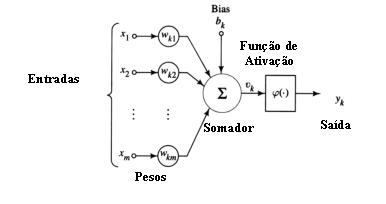
\includegraphics[scale=0.7]{pasta1_figuras/neuronio_artificial.jpg}
    \caption{Neurônio Artificial}
\end{figure}

Como nos neurônios presentes no sistema nervoso, o neorônio artificial possui um meio de recepção dos estimulos vindos do meio externo, que são denominadas as entradas. Os pesos são atribuidos a cada entrada e estes podem sofrer alteração durante o processo de treinamento. O somador obtem o resultado da soma das multiplicações das entradas pelos pesos e transmite o potencial de ativação à função de ativação. A função de ativação aplicará a saída do somador em alguma função especifica obtendo assim, a saída da rede neural.

As topologias e arquiteturas de uma rede neural são definidas sob algumas especificações. Tais são elas: direção de fluxo de dados, tipo de aprendizado, algoritmo de aprendizado e a realimentação, disposição espacial dos neurônios.

Arquiteturas feedfoward processam os dados em direção a saída, ou seja, a partir da camada de entrada o processamento dos dados ocorrerá de camada em camada, passando por todas as camadas escondidas até chegar na camada de saída. Um exemplo genérico de uma arquitetura feedfoward pode ser visto na figura a seguir:
\begin{figure}[h]
	\centering
    \label{fig1}
    \vspace{3ex}%
	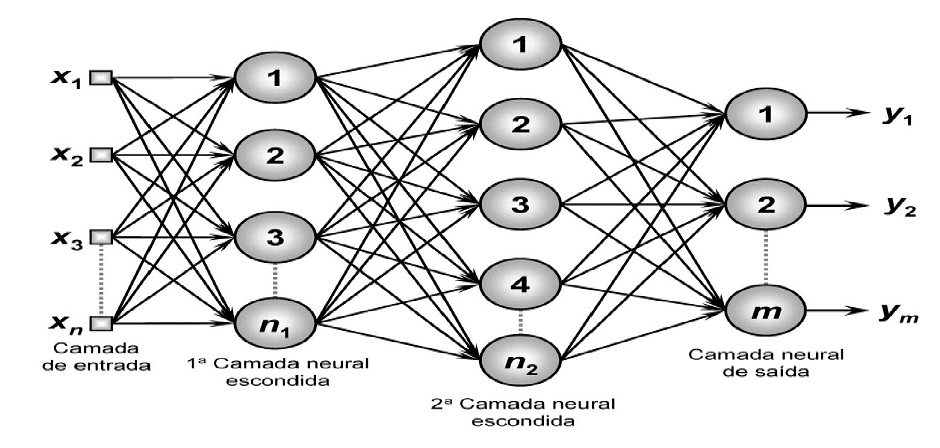
\includegraphics[scale=0.4]{pasta1_figuras/rna-Feedfoward.png}
    \caption{Neurônio Artificial}
\end{figure}

Em algumas arquiteturas é possível encontrar também interconexões das camadas no sentido da camada de saída em direção a camada de entrada. Tal arquitetura é denominada recorrente. Um exemplo dessa topologia pode ser observada na figura 2.3.
\begin{figure}[h]
	\centering
    \label{fig1}
    \vspace{3ex}%
	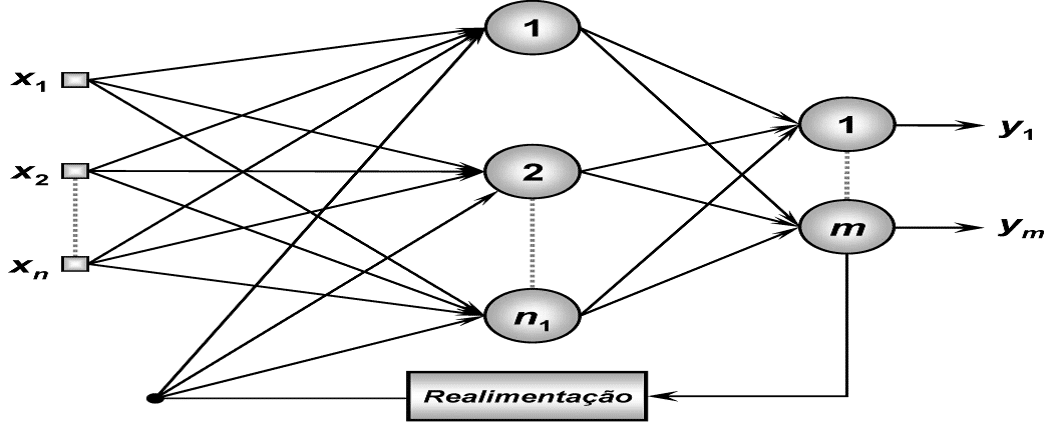
\includegraphics[scale=0.35]{pasta1_figuras/redes-recorrentes.png}
    \caption{Neurônio Artificial}
\end{figure}

Um dos conceitos fundamentais no projeto de redes neurais artificiais é o treinamento. O treinamento possui a função de ajustar os pesos da rede fazendo com que a mesma seja capaz de generalizar o aprendizado. Existem dois tipos de treinamento: Supervisionado e não supervisionado. O treinamento supervisionado é feito com o auxílio de um professor, ou seja, para um determinado conjunto de entradas existe uma saída conhecida e desejada. O aprendizado no treinamento não supervisionado será feito sem "professor" reconhecendo padrões, relações e regularidades sem conhecer as saídas.

Dentre os diversos algoritmos, destaca-se o backpropagation pela sua capacidade de resolver problemas não-linearmente separáveis. Este algoritmo só é aplicável em arquiteturas multicamadas e o seu processo de ajustes de pesos se baseia na retro propagação do erro. A perceptron multicamada é uma das arquiteturas que utiliza deste algoritmo de treino para generalizar suas soluções não-linearmente separáveis. Um exemplo de PMC pode ser visto a seguir:
\begin{figure}[h]
	\centering
    \label{fig1}
    \vspace{3ex}%
	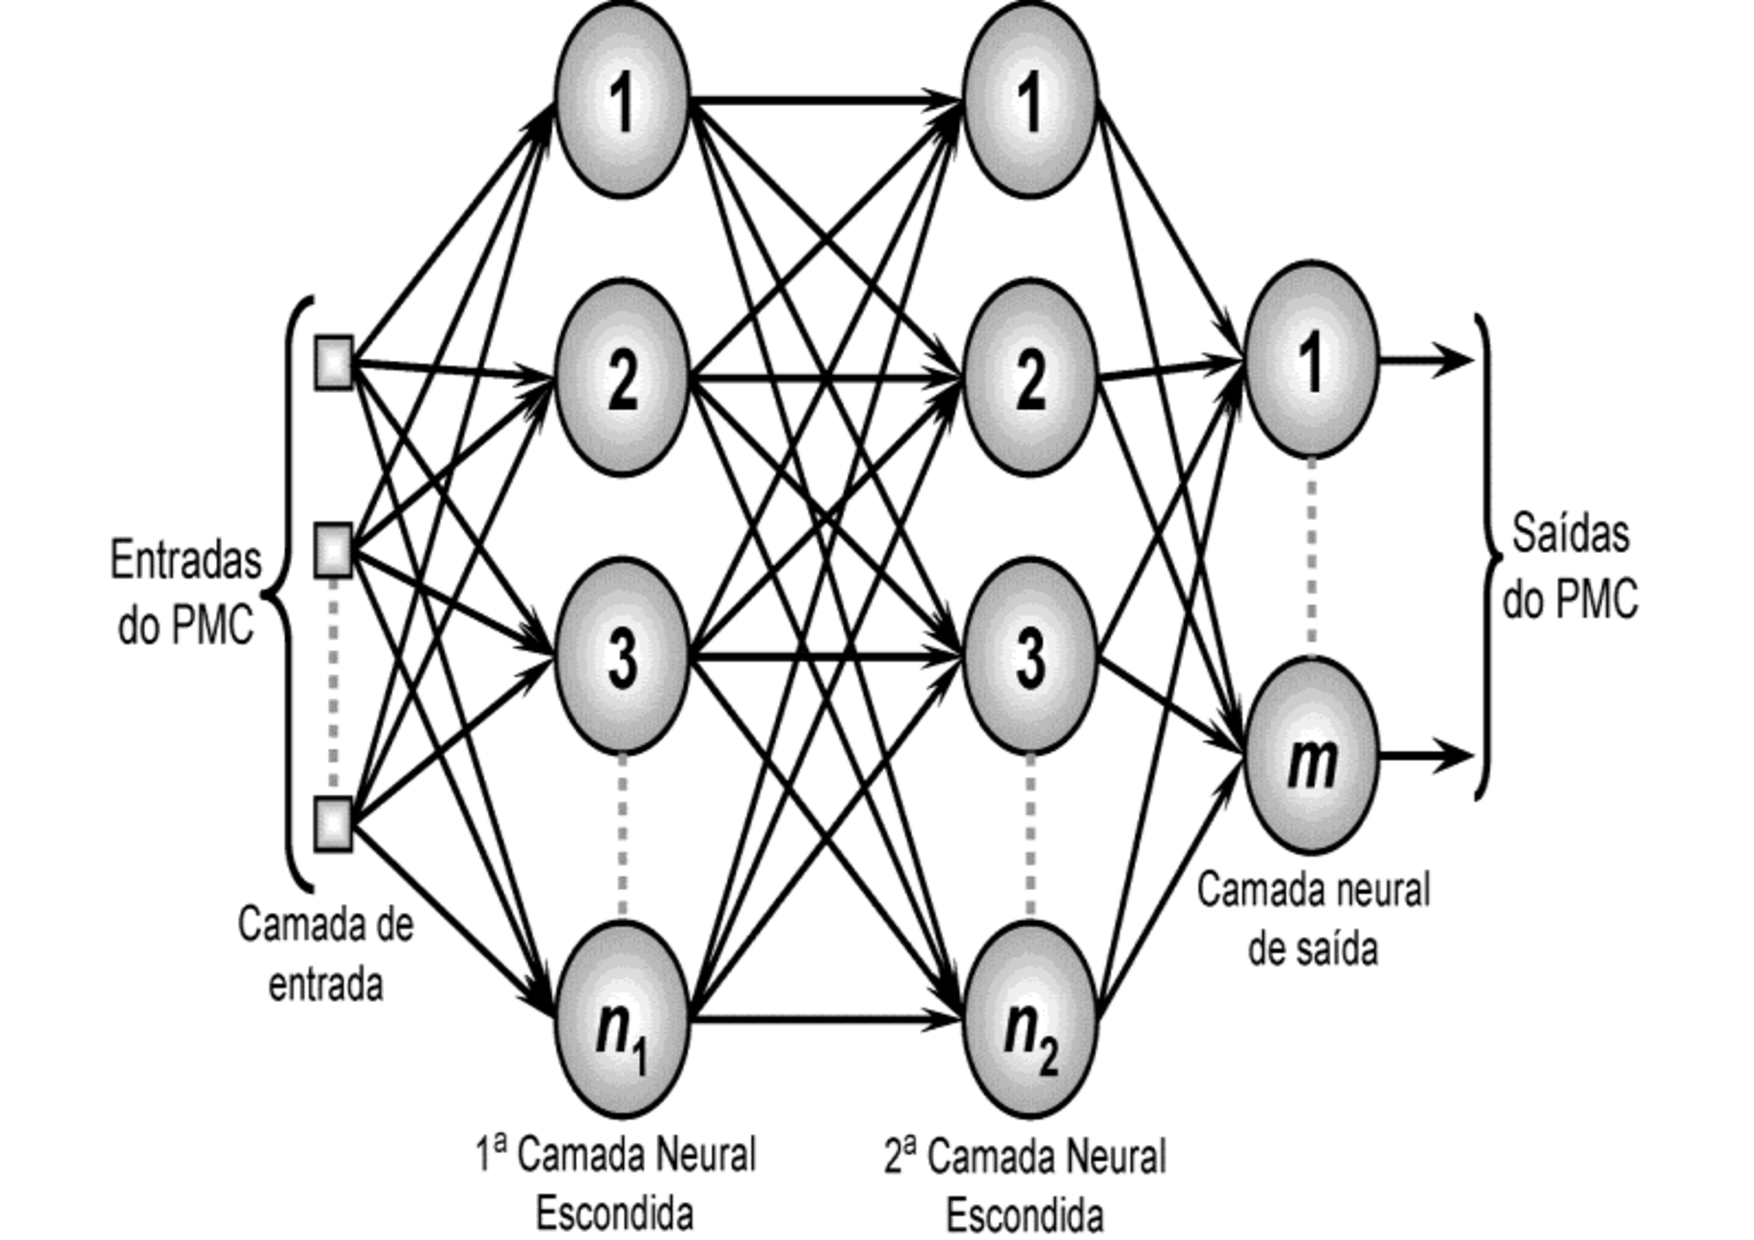
\includegraphics[scale=0.4]{pasta1_figuras/pmc.pdf}
    \caption{Neurônio Artificial}
\end{figure}

Overfitting e underfitting são classificações sobre a capacidade de generalização da rede. O overfitting ocorre quando a rede recebe treinamento demasiado das amostras do dataset, e no contrário, quando o treinamento é insuficiente ocorre o underfitting da capacidade de generalização. Para validar se uma rede neural já atende as especificações ótimas de generalização, ou seja, o ponto ótimo entre o overfitting e o underfitting. Alguns métodos de validação e testes já são utilizados no processo de treinamento de uma rede neural. Um muito conhecido é o método da validação cruzada, onde o dataset é dividido em 3 subconjuntos de amostras: Treino, validação e teste. O subconjunto do treino será o conjunto que treinará os pesos dos neurônios. Sob as amostras de validação serão calculados o erro até que se alcance a condição de parada. E por fim, o subconjunto de teste será usado para estipular os parametros da capacidade de generalização da rede. Na validação cruzada os subconjuntos de treino serão divididos em k partes iguais, onde cada k parte será o conjunto de validação durante uma certa quantidade de épocas de treino.
\subsection{Verificação}
Verificação é um método utilizado para verificar a corretude de uma certa propriedade sob o funcionamento de um sistema. Tal técnica viza a validação e a confiabilidade de uma propriedade específica. Verificação formal se divide em dois tipos de abordagens: a verificação dedutiva e a verificação de modelos. No caso da primeira abordagem, a verificação permite a prova de propriedades temporais em sistemas com estados infinitos. Já na segunda abordagem, a verificação de modelos, do inglês \textit{Model Checking}, trata do problema de testar de forma automática se um modelo de um determinado sistema atende a uma respectiva especificação, sendo que, por exemplo, tais especificações podem estar relacionadas com as propriedades de segurança e/ou de vivacidade do sistema em questão. Para solucionar este problema de forma algorítmica, é representado matematicamente o sistema e suas especificações utilizando métodos formais, como por exemplo, Lógica Proposicional e Lógica Temporal Linear, de tal forma que se possa verificar se uma dada fórmula é satisfeita dada uma determinada estrutura \cite{jhala2009}.

A expressão "verificação de modelos"  se refere a um algoritmo que explora o espaço de estados de um sistema a fim de verificar propriedades. Este também verifica se as transições dos estados respeitam as restrições impostas pelo sistema \cite{clarke2001}.  Tal algoritmo realiza uma verificação exaustiva no espaço de estados de maneira automática em busca de uma violação de restrição.


Um dos principais problemas enfrentados pelas técnicas de verificação de modelos até hoje é a explosão de estados. Tal problema ocorre quando os estados da estrutura obtida a partir do sistema em questão crescem exponencialmente \cite{clarke2001}. Embora, muitos ganhos já foram obtidos em relação a eficiência dos verificadores, a explosão de estados ainda é um problema crítico para as ferramentas hoje existentes.


Ferramentas de software que executam a técnica de verificação automática são chamadas de verificadores. Esses se baseiam nas teorias da verificação de modelos, que possuem o objetivo de verificar de maneira rápida e eficiente propriedades de um código. Com o crescimento da verificação formal em sistemas de software , muitas ferramentas foram desenvolvidas para verificar propriedades não usuais para diversos frameworks presente no mercado. A verificação de corrida de dados em gpus é um exemplo que algumas ferramentas já verificam. Algumas destas são: ESBMC-GPU \cite{monteiro2018}, Gklee \cite{gklee}, GPUVerify \cite{gpuverify}, etc. 


O desenvolvimento desse projeto gira em torno do verificador ESBMC-GPU \cite{monteiro2018}, um verificador que é capaz de verificar as propriedades: estouro aritméticos de vetores, ponteiros nulos, corrida de dados, divisão por zero e assertivas definidas pelo usuário. Este verificador utiliza das técnicas da verificação de modelos e possui algumas características particulares.  


O ESBMC aplica técnicas de BMC (\textit{Bounded Model Checking}) baseado em SMT (\textit{Satisfiability Modulo Theories}) para verificar programas C/C++, e da linguagem CUDA, usada para programação de GPU. A técnica BMC possui a ideia básica de checar a negação de uma propriedade até uma determinada profundidade. Dado um sistema de transição de estados M, uma propriedade $\phi$, e um limite k, BMC desdobra o sistema k vezes e o traduz para uma condição de verificação (\textit{verification condition}, VC) $\Psi$, tal que $\Psi$ é satisfatíel, se e somente se, $\phi$ possuir um contraexemplo de profundidade k ou menor \cite{cordeiro2012}.


SMT resolve as fórmulas de satisfatibilidade de primeira ordem usando a combinação de diferentes teorias e assim generaliza a satisfatibilidade proposicional por suportar funções não interpretadas, aritmética linear e não linear, vetores de bit, tuplas, arrays, e outras teorias de primeira ordem.


O ESBMC-GPU tem como base um algoritmo de exploração preguiçosa, que no lugar de verificar de uma única vez todas as possíveis intercalações de um programa, verifica de forma incremental uma intercalação por vez \cite{cordeiro2011}. O algoritmo percorre, em profundidade, a árvore de alcançabilidade de estados (\textit{Reachability Tree}, RT). Ao chegar em um nó folha, o algoritmo passa para o solucionador uma fórmula SMT que representa uma intercalação específica do programa CUDA. Caso esta fórmula seja satisfatível, uma violação da propriedade no programa CUDA foi encontrada e, assim, um contraexemplo é fornecido. Caso contrário, é realizado um \textit{backtrack} na RT e uma nova intercalação é produzida e verificada pelo solucionador SMT. O algoritmo termina quando ou uma violação é encontrada pelo ESBMC ou todas as intercalações foram verificadas com sucesso.


Além do algoritmo de exploração preguiçosa o ESBMC-GPU ainda utiliza da técnica MPOR (\textit{Monotonic Parcial Order Reduction}). Tal técnica é utilizada para reduzir as intercalações redundantes \cite{kahlon2009}. O algoritmo classifica as transições dentro de um programa multitarefa que são independentes ou dependentes de transições em outras threads, objetivando determinar se pares de intercalações sempre computam o mesmo estado, descartando os estados da RT que são duplicados \cite{morse2015}.


\subsection{CUDA}

CUDA é uma plataforma de computação paralela de propósito geral que representa um modelo de programação desenvolvido pela empresa NVIDIA para executar em GPUs fabricadas pela mesma. É uma linguagem desenvolvida para ter uma rápida curva de aprendizado, cujo o ambiente pode ser facilmente utilizado por programadores das linguagens C/C++ e/ou Fortran [NVIDIA 2015].

No modelo de programação de CUDA, o conceito de kernel é usado para uma função que executa n cópias paralelamente na GPU, onde n é o produto do número de blocos e threads. Um kernel é definido por um especificador \textunderscore\textunderscore global\textunderscore\textunderscore  e sua chamada no programa é feita pela notação kernel\textless\textless\textless B,T\textgreater\textgreater\textgreater, onde B é o número de blocos e T é o número de threads. Cada kernel é referenciado na GPU como thread e cada thread recebe um identificador único (ID) formado pelo número da thread e o número do bloco. O ID da thread é usado para indexar as suas tarefas (i.e., posições de memória e cooperação). As threads são organizadas em blocos.


Dentro de um bloco, a hierarquia de threads é definida pela variável chamada threadIdx. Esta variável é um vetor de três componentes permitindo usar índices uni-, bi- e tridimensionais. Por exemplo, para obter o ID de uma thread nestas configuraçõe para um bloco bidimensional de tamanho (Dx,Dy), o ID da thread de índice (x,y) e obtido por (x+yDx), e para um bloco tridimensional de tamanho (Dx,Dy,Dz), a ID de uma thread de índice (x, y, z) é definido por (x + yDx + zDxDy) [NVIDIA 2015].


Os blocos também podem ser definidos em trê dimensões, onde cada dimensão pode ser acessada pela variável blockIdx. Esta variável também é formada por três componentes permitindo usar blocos uni-, bi- e tridimensionais. O número máximo de threads por bloco depende da geração da placa variando de 1024 a 2048 [NVIDIA 2015]. Os blocos possuem a característica de serem executados em qualquer ordem, podendo ser alocados a qualquer processador. Com isso, um kernel pode ser executado por mútiplos blocos de forma igual, e o número total de threads é o número de blocos vezes o número de threads por bloco.


Um conceito utilizado na programação de CUDA, é fazer referência a GPU como device e a unidade de processamento central (CPU) como host.     device é um especificador para funções que executam e são chamadas somente pela GPU, e host para funções que executam e são chamadas somente pela CPU. O fluxo comum da alocação de dados para o device é feito no host usando as funções cudaMalloc, cudaFree e cudaMemcpy. Estas são funções essenciais para um programa CUDA, pois os dados são transferidos do host para o device e vice-versa. A função cudaMalloc aloca uma quantidade de memória no device, a qual é liberada após sua utilização pela função cudaFree. A função cudaMemcpy é usada para copiar dados inicializados no host para o device. Suas interfaces são baseadas nas funções malloc, free e memcpy da linguagem C.

Devido a eficiência do paralelismo das aplicações desenvolvidas em CUDA e em outras plataformas que operam nas GPUs de forma genérica, muitos ganhos foram obtidos em paralelizar operações. Um exemplo pode ser visto no comparativo de multiplicação de matrizes esparsas entre GPUs e CPUs em \cite{liang2017}.

APIs voltadas apenas para cálculo de matrizes e primitivas de ANNs surgiram nos últimos anos. CUblas e CUdnn são exemplo dessas APIs e foram desenvolvidas em CUDA pela empresa NVIDIA. Tais APIs possuem funções que executam diversas operações de forma paralela nas threads dos dispositivos \textit{many-cores}.

As ANNs são ,na maioria das vezes, sistemas que podem ser modelados por matrizes, e suas operações são baseadas majoritariamente em produtos e somas. Além dessas operações básicas, as ANNs também possuem funções de ativações especificas, podendo algumas até possuir camadas de convolução e \textit{pooling} que são muito utilizadas em reconhecimento de imagens \cite{Kim2017}. CUDNN e CUBLAS, trazem justamente esse \textit{gap}, onde os produtos e somas das matrizes, as primitivas funções das ANNs e operações de convolução e \textit{pooling} são executadas utilizando do paralelismo das GPUs \cite{wang2015}. 

\section{Trabalhos Relacionados}
% Fim Capítulo

Por ser um tema relativamente atual, a verificação de ANN já é uma área de pesquisa muito visada. As técnicas utilizadas neste projeto se baseiam nos seguintes trabalhos relacionados:

Em \cite{reluplex}, é proposto um verificador de ANNs voltadas para a função de ativação Relu. Este utiliza do método simplex \cite{Bartels1971} para poluir as amostras a serem verificadas. As contribuições são: (i) Reluplex, um SMT solver para a teoria da linear real arithmetic com ReLU constraints. (ii) Mostrar como DNNs e as propriedades de interesse podem ser codificadas como entradas para o Reluplex. (iii) discutir vários detalhes de implementações que são cruciais para performance e escalabilidade, como a aritmetica de ponto flutuante, limites de derivação para as variáveis ReLU e análise de conflitos. (iv) conduzir uma completa avaliação na implementação do protótipo ACAS XU system, demonstrando a habilidade escalável do Reluplex em DNNs que são maiores em ordem de magnitude que as outras que podem ser analizadas usando técnicas existentes.


 Em \cite{marta2016} é proposto um \textit{framework} de verificação para \textit{feed-forward multi-layer neural networks} baseadas em SMT. Este foca na segunraça das decisões nos reconhecimentos de imagens com respeito a manipulação de imagens, como por exemplo: arranhões, mudanças no ângulo da câmera e condições de luminosidade que resultariam no mesmo resultado classificado por um humano. A técnica utilizada se baseia numa busca exaustiva de uma região empregando discretização e propagando a analise camada por camada. O método lida diretamente com o código da ANN e pode garantir que os exemplos adversos, se existem, são encontrados pela dada região. As técnicas foram implementadas utilizando o SMT solver Z3\cite{z3}.
 
 Em \cite{kroening2018} é proposto uma metodologia de como testar a segurança de ANNs em dominios críticos. A metodologia se baseia no trdicional MC/DC \textit{coverage criterion} \cite{chang2007}. Os criterios de avaliação são incomparáveis e interdependentes. É proposto um algoritmo para geração de casos de teste baseado em LP (\textit{linear programming}, onde um novo caso de teste é obtido a partir de pertubações inseridas em outros casos de teste. Os métodos visam 4 objetivos: (1) busca de bugs; (2) métrica de segurança para DNNs; (3) eficiência do teste; (4) analise das estruturas internas de DNNs.
 
 
 
 
 
 
\chapter{Verificação de Modelos Aplicado a Redes Neurais Implementadas em CUDA} \label{cap3}
MODELAGEM AQUI
% Fim Capítulo

\chapter{ESBMC-GPU e Modelos Operacionais} \label{cap4}
METODOLOGIA AQUI

% Fim Capítulo
\chapter{Aplicação Experimental} \label{cap5}
\section{Objetivos Experimentais}
\section{Descrição dos Experimentos}
\section{Ambiente Experimental}
\section{Resultados}
RESULTADOS AQUI
% Fim Capítulo

\chapter{Conclusão} \label{cap6}
\section{Conseiderações Finais}
\section{Trabalhos Futuros}
CONCLUSÃO AQUI

% Fim Capítulo


% FOI RENOMEADO O ARQUIVO: main_tcc.bbl para main_tcc.bbl_OLD
\bibliographystyle{IEEEtranN} % Ordem de citação
%\bibliographystyle{humannat} % Ordem alfabética
%\bibliographystyle{dinat}    % Ordem alfabética
%\bibliographystyle{plainnat} % Ordem alfabética
%\bibliographystyle{apa}      % Ordem alfabética

\bibliography{referencias}
\appendix

%\chapter{TITULO APÊNDICE} \label{apendice:a}




\end{document}